% kapitel2.tex
%\chapter{Die Softwarekonstruktion}
%\label{chapter:kap2}
\section{Aufbau der Softwarearchitektur}
Wie im vorherigen Teil der Ausarbeitung verdeutlicht wurde, bildet der Raspberry Pi im inneren des Spiegels das Kernstück der gesamten Plattform. Aus diesem Grund läuft die gesamte entwickelte Software auf entsprechendem Modul. 

Dabei ist das Softwareprojekt in zwei Programmteile aufgeteilt. Das erste Programm beinhaltet die benötigte Kommunikation und Erzeugung der UI für den SmartMirror. Dabei ist dieses Programm in Python geschrieben und hat die Hauptarbeit in Anspruch genommen, wo hingegen das zweite Programm ein Skript umfasst, das nach dem Systemstart das eigentliche SmartMirror Programm startet. 

\begin{figure}
	\centering
	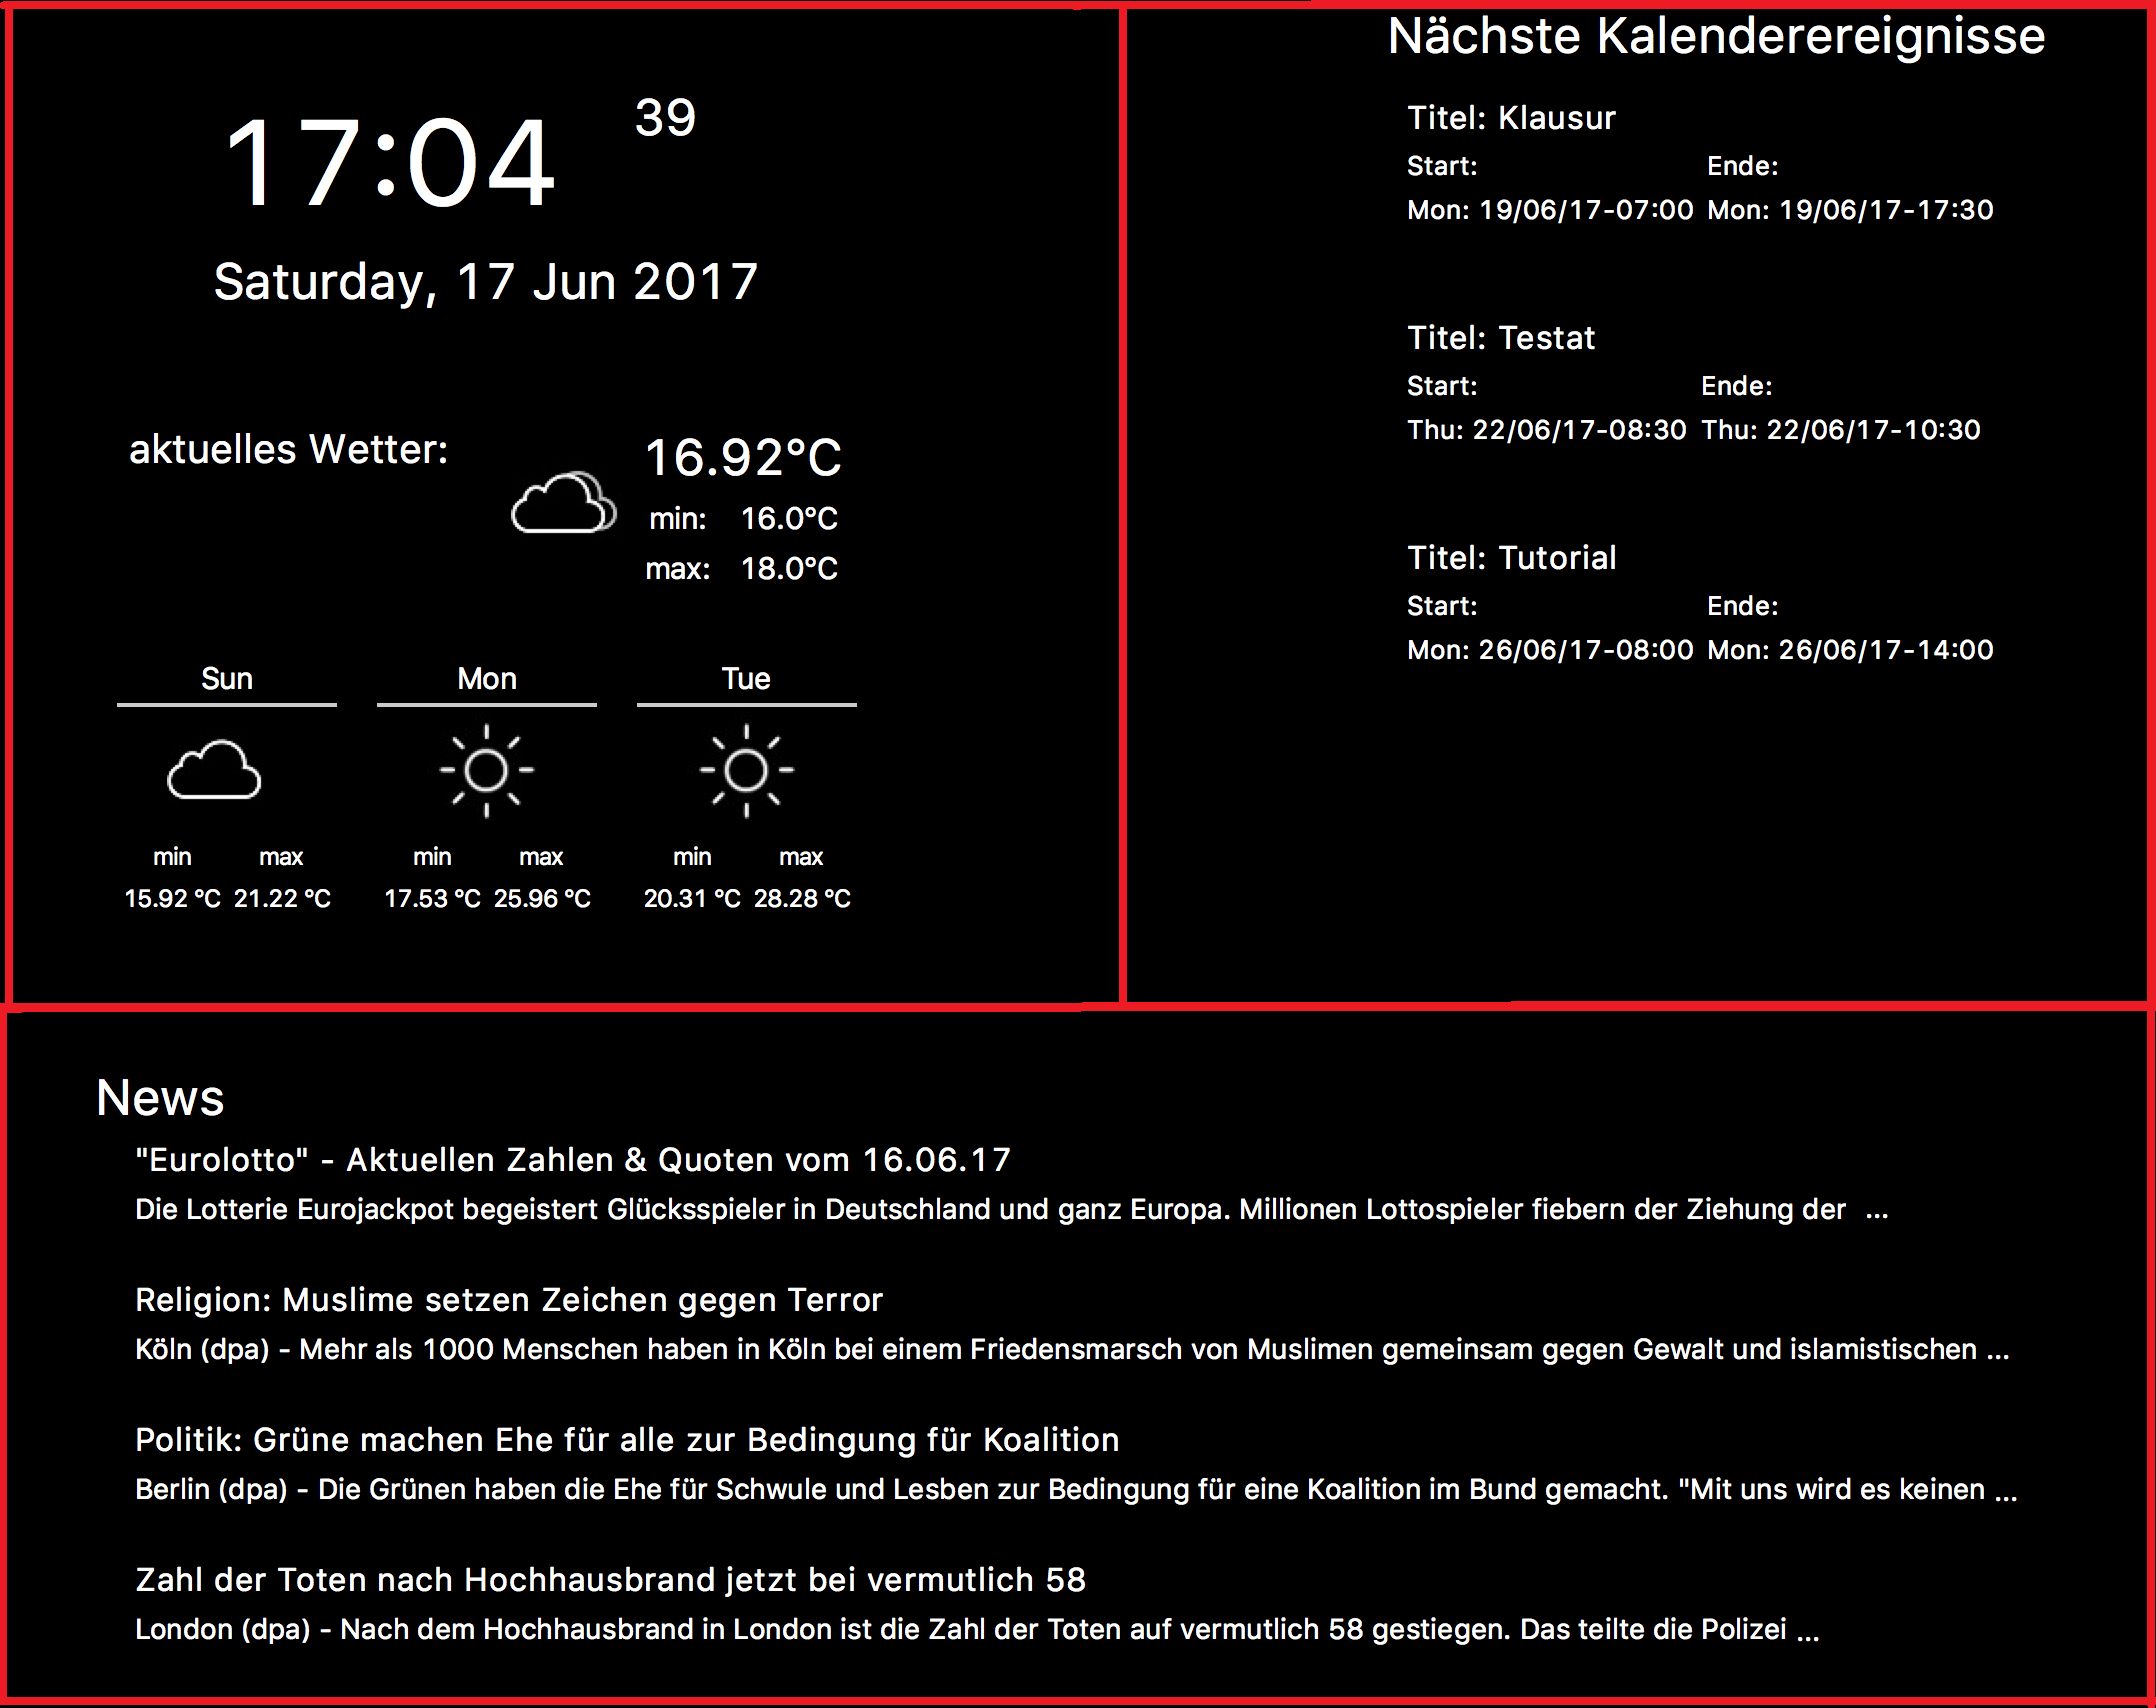
\includegraphics[width=0.7\linewidth]{bilder/grafOberflaeche}
	\caption[UI der SmartMirror Applikation]{UI der SmartMirror Applikation}
	\label{fig:grafoberflaeche}
\end{figure}

\begin{figure}
	\centering
	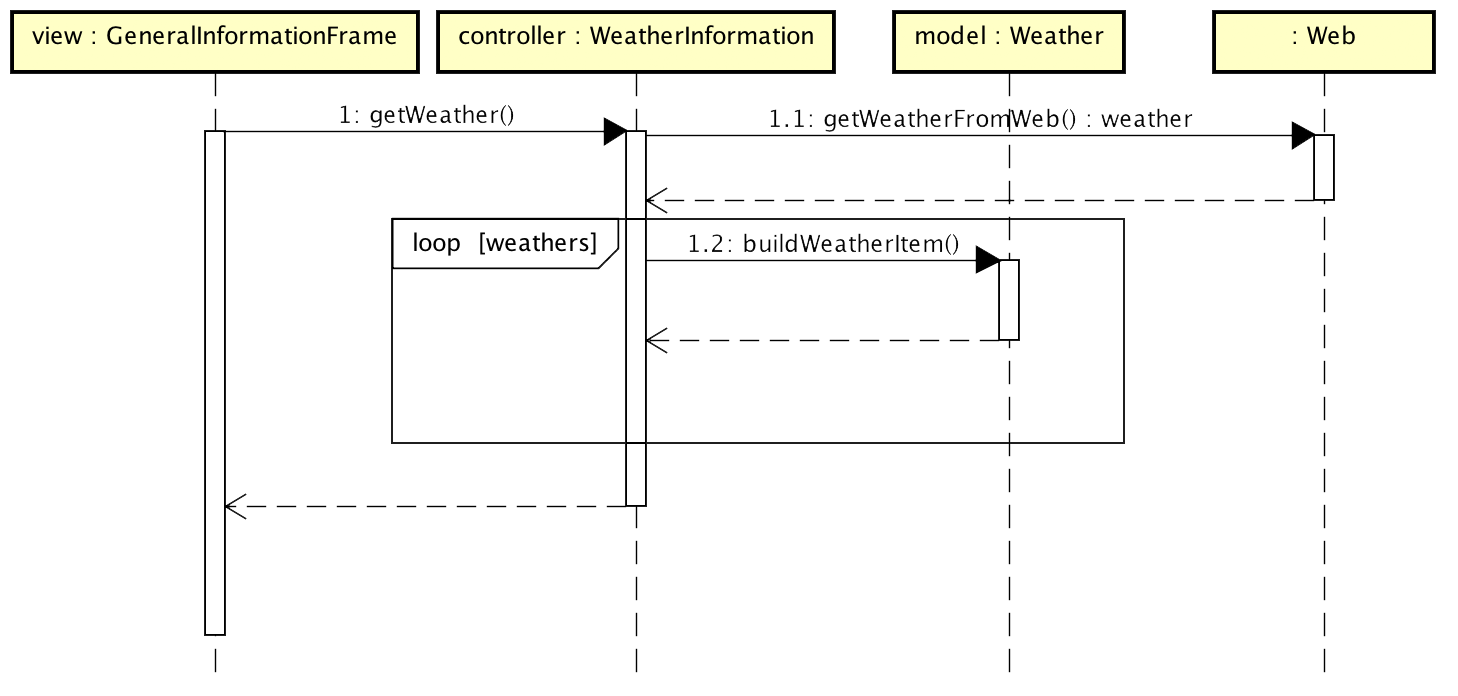
\includegraphics[width=0.7\linewidth]{bilder/sequenceDiagramGettingDataNoBackground}
	\caption{Sequenzdiagramm: Bezug von Daten aus dem Internet}
	\label{fig:sequenzDiagramData}
\end{figure}

\begin{figure}
	\centering
	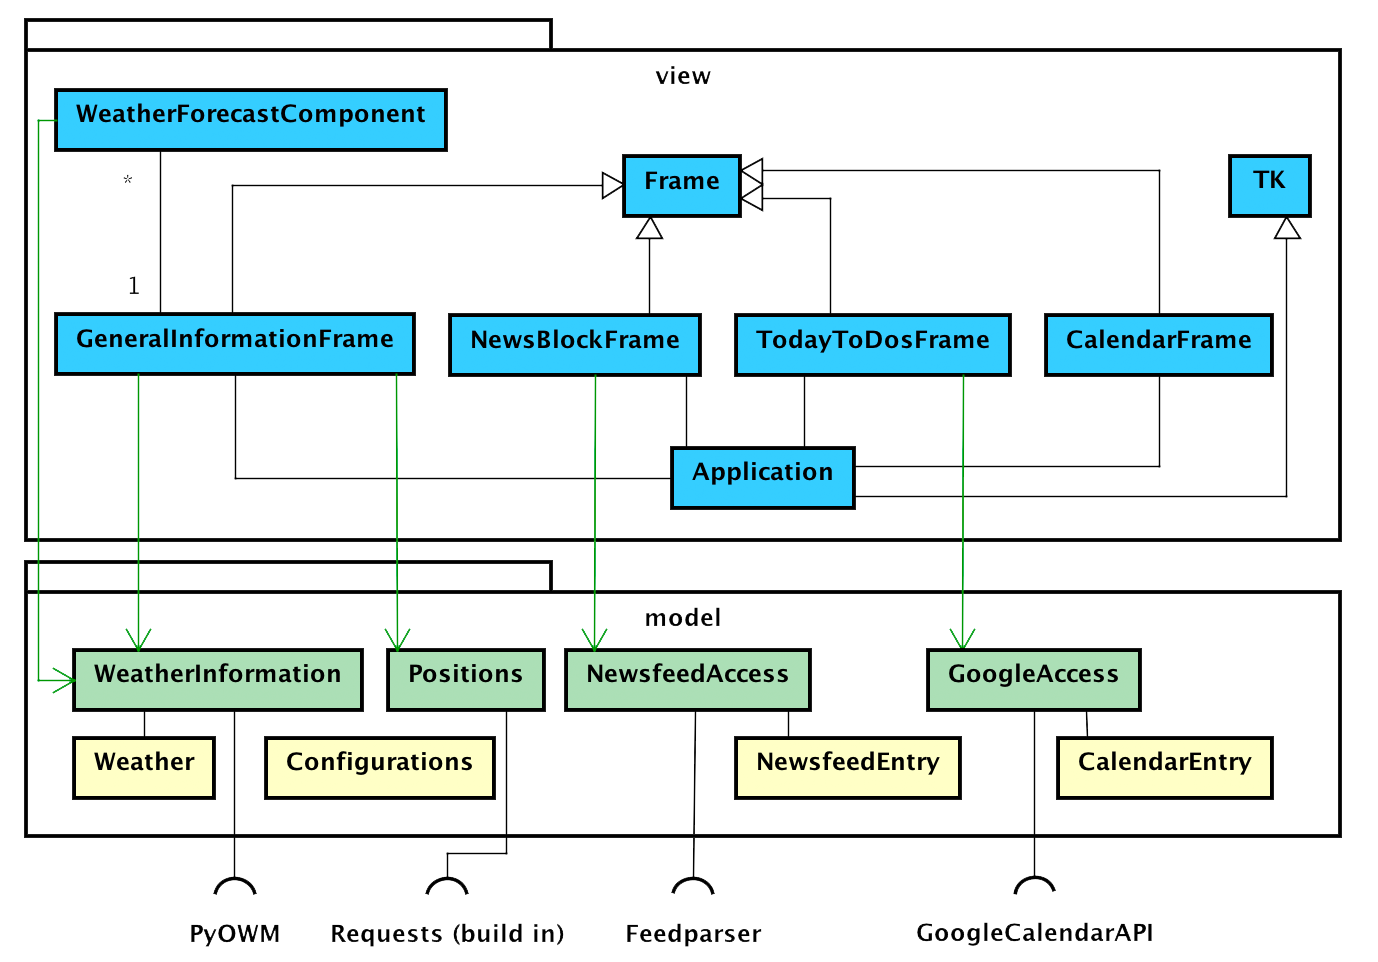
\includegraphics[width=0.7\linewidth]{bilder/umlDiagramNoBackground}
	\caption[UML-Diagramm: Klassenaufbau der Hauptapplikation]{UML-Diagramm: Klassenaufbau der Hauptapplikation}
	\label{fig:umldiagramClasses}
\end{figure}

Die vom Hauptprogramm erzeugte UI wird in \autoref{fig:grafoberflaeche} dargestellt

\subsection{Eingebettete Libraries}

\subsection{Kommunikation mit externen Systemen}

\subsection{Ausimplementierung der Applikation}